\documentclass[tikz,border=10pt,12pt]{standalone}
\usetikzlibrary{arrows.meta, positioning, calc, decorations.pathreplacing}
\usepackage{amsmath}
\usepackage{amssymb}

\begin{document}
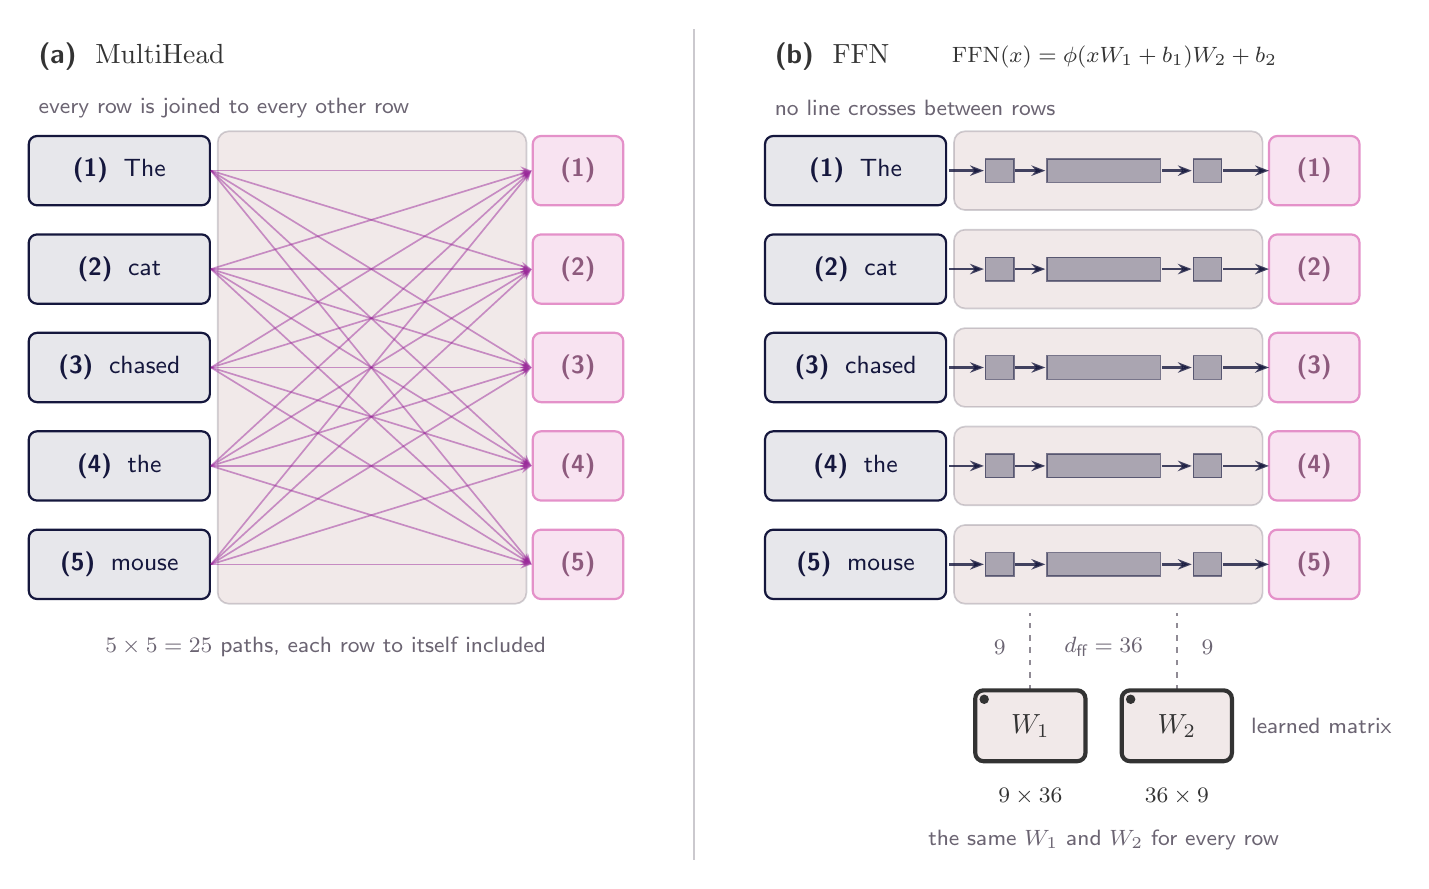
\begin{tikzpicture}[
    every node/.style={font=\sffamily},
]

\definecolor{c1}{HTML}{15173D}
\definecolor{c2}{HTML}{982598}
\definecolor{c3}{HTML}{E491C9}
\definecolor{c4}{HTML}{F1E9E9}
\definecolor{axiscolor}{HTML}{333333}
\definecolor{labelcolor}{HTML}{6B6472}

% ================================================================
% VISUAL GRAMMAR
%   computed tensor : thin outline, tinted fill
%   learned matrix  : thick outline + corner dot   (as attention_breakdown)
%
% The two panels are the SAME layout with two things swapped: what fills
% the middle region, and how many arrows cross it.
%
% LEGIBILITY BUDGET.  The page renders this at 768 px, so what matters is
% the ratio of type size to total width, not either one alone.  The class
% is 12pt and the cm grid is tight, which is the whole trick: the drawing
% is ~521 pt wide, so 768 px means a 1.47x upscale on the page.
%   \normalsize 12    -> ~17.7 px   panel titles, W_1 and W_2
%   \small      10.95 -> ~16.1 px   row labels
%   \footnotesize 10  -> ~14.7 px   every annotation, nothing below this
% All three are native Computer Modern sizes, so no size substitution.
%
% Panel origin:  (a) o = 0.00     (b) o = 9.35     divider at x = 8.45
% Everything below is written o + dx, so the two panels are congruent.
%
%   dx  0.00 .. 2.30   the five row boxes   (centre o+1.15, width 2.30)
%   dx  2.40 .. 6.32   the middle region    (identical extent in both)
%   dx  6.40 .. 7.55   the five out boxes   (centre o+6.975, width 1.15)
%
% Rows, identical y in both panels, 1.25 apart, boxes 0.88 tall:
%   (1) 5.00   (2) 3.75   (3) 2.50   (4) 1.25   (5) 0.00
% Bands are 1.00 tall, so 0.25 of clear air stays between neighbours.
%
% (a) the middle region is ONE block of c4 with all 25 c2 arrows in it.
% (b) the middle region is FIVE bands of c4, one per row, never touching.
%
% Panel (b) lane content, dx from o, bars 0.30 tall centred on the row:
%   2.34 -> 2.78  arrow
%   2.80 .. 3.16  bar of width  9   (0.36 long)
%   3.18 -> 3.56  arrow, W_1 tie at dx = 3.37
%   3.58 .. 5.02  bar of width 36   (1.44 long, exactly 4x)
%   5.04 -> 5.42  arrow, W_2 tie at dx = 5.23
%   5.44 .. 5.80  bar of width  9
%   5.82 -> 6.40  arrow
% W_1 and W_2 sit below the stack with short dashed stubs that stop under
% the bottom band. Nothing vertical crosses the lanes, so no mark in (b)
% can be mistaken for a connection between rows; "shared" is carried by
% drawing the two matrices once and by the note at y = -3.50.
%
%   y  6.45  panel titles          y  5.80  panel subtitles
%   y -1.05  the three widths      y -2.05  W_1, W_2 and the legend key
%   y -2.95  their shapes          y -3.50  the sharing note
% ================================================================

\def\oA{0.00}
\def\oB{9.35}
\def\bandL{2.40}
\def\bandR{6.32}
\def\hh{0.50}          % half height of a lane band
\def\bh{0.15}          % half height of a width bar

\tikzset{
  rowbox/.style={draw=c1, line width=0.8pt, fill=c1, fill opacity=0.10,
    text opacity=1, rounded corners=3pt, minimum width=2.3cm,
    minimum height=0.88cm, font=\sffamily\small, text=c1, inner sep=2pt},
  outbox/.style={draw=c3, line width=0.8pt, fill=c3, fill opacity=0.26,
    text opacity=1, rounded corners=3pt, minimum width=1.15cm,
    minimum height=0.88cm, font=\sffamily\small, text=c3!62!black},
  learn/.style={draw=axiscolor, line width=1.5pt, fill=c4, text opacity=1,
    rounded corners=3pt, minimum width=1.40cm, minimum height=0.90cm,
    font=\sffamily\normalsize, text=axiscolor},
  band/.style={fill=c4, draw=labelcolor, draw opacity=0.30, line width=0.6pt,
    rounded corners=4pt},
  mesh/.style={-{Stealth[length=4pt]}, line width=0.6pt, c2, opacity=0.48},
  lane/.style={-{Stealth[length=5pt]}, line width=1.0pt, c1, opacity=0.80},
  tie/.style={labelcolor, opacity=0.75, line width=0.8pt, dash pattern=on 2pt off 2.5pt},
  ttl/.style={font=\sffamily\normalsize\bfseries, text=axiscolor, anchor=west},
  sub/.style={font=\sffamily\footnotesize, text=labelcolor, anchor=west},
  wlab/.style={font=\sffamily\footnotesize, text=labelcolor},
  shp/.style={font=\sffamily\footnotesize, text=axiscolor},
  note/.style={font=\sffamily\footnotesize, text=labelcolor},
}

\newcommand{\dotmark}[1]{\fill[axiscolor] ($(#1.north west)+(0.14,-0.14)$)
    circle (0.06);}

% ---------------------------------------------------------------- titles
\node[ttl] at (\oA, 6.45) {(a)\; $\mathrm{MultiHead}$};
\node[sub] at (\oA, 5.80) {every row is joined to every other row};

\node[ttl] at (\oB, 6.45) {(b)\; $\mathrm{FFN}$};
\node[sub] at (\oB, 5.80) {no line crosses between rows};
\node[font=\sffamily\footnotesize, text=axiscolor, anchor=west] at (\oB+2.25, 6.45)
    {$\mathrm{FFN}(x) = \phi(x W_1 + b_1) W_2 + b_2$};

% ---------------------------------------------------------------- divider
\draw[labelcolor, opacity=0.35, line width=0.9pt] (8.45, -3.75) -- (8.45, 6.80);

% ================================================================
% (a)  one region, twenty-five paths
% ================================================================
\foreach \i/\y/\w in {1/5.00/The, 2/3.75/cat, 3/2.50/chased, 4/1.25/the, 5/0.00/mouse} {
    \node[rowbox] (ain\i) at (\oA+1.15, \y) {\textbf{(\i)}\; \w};
    \node[outbox] (aout\i) at (\oA+6.975, \y) {\textbf{(\i)}};
}

\fill[band] (\oA+\bandL, -\hh) rectangle (\oA+\bandR, 5.00+\hh);

\foreach \i in {1,...,5} {
    \foreach \j in {1,...,5} {
        \draw[mesh] (ain\i.east) -- (aout\j.west);
    }
}

% one annotation line, on the same y as the widths of panel (b), so the
% two panels stay registered below the rows as well as beside them
\node[note] at (\oA+3.77, -1.05) {$5 \times 5 = 25$ paths, each row to itself included};

% ================================================================
% (b)  five lanes, five paths
% ================================================================
% short stubs only: they stop below the bottom band, so no mark ever
% crosses the lane stack and nothing can be read as a row-to-row path
\draw[tie] (\oB+3.37, -1.60) -- (\oB+3.37, -0.62);
\draw[tie] (\oB+5.23, -1.60) -- (\oB+5.23, -0.62);

\foreach \i/\y/\w in {1/5.00/The, 2/3.75/cat, 3/2.50/chased, 4/1.25/the, 5/0.00/mouse} {
    \node[rowbox] (bin\i) at (\oB+1.15, \y) {\textbf{(\i)}\; \w};
    \node[outbox] (bout\i) at (\oB+6.975, \y) {\textbf{(\i)}};

    \fill[band] (\oB+\bandL, \y-\hh) rectangle (\oB+\bandR, \y+\hh);

    % width 9 -> width 36 -> width 9, the bars drawn to scale
    \foreach \bl/\br in {2.80/3.16, 3.58/5.02, 5.44/5.80} {
        \fill[c1, opacity=0.32]
            (\oB+\bl, \y-\bh) rectangle (\oB+\br, \y+\bh);
        \draw[c1, opacity=0.55, line width=0.5pt]
            (\oB+\bl, \y-\bh) rectangle (\oB+\br, \y+\bh);
    }
    \draw[lane] (\oB+2.34, \y) -- (\oB+2.78, \y);
    \draw[lane] (\oB+3.18, \y) -- (\oB+3.56, \y);
    \draw[lane] (\oB+5.04, \y) -- (\oB+5.42, \y);
    \draw[lane] (\oB+5.82, \y) -- (\oB+6.40, \y);
}

% the three widths, named once, under the bottom lane
\node[wlab] at (\oB+2.98, -1.05) {$9$};
\node[wlab] at (\oB+4.30, -1.05) {$d_{\text{ff}} = 36$};
\node[wlab] at (\oB+5.62, -1.05) {$9$};

% the two shared matrices, drawn once
\node[learn] (W1) at (\oB+3.37, -2.05) {$W_1$};  \dotmark{W1}
\node[learn] (W2) at (\oB+5.23, -2.05) {$W_2$};  \dotmark{W2}
\node[shp] at (\oB+3.37, -2.95) {$9 \times 36$};
\node[shp] at (\oB+5.23, -2.95) {$36 \times 9$};
\node[note] at (\oB+4.30, -3.50) {the same $W_1$ and $W_2$ for every row};

% ---------------------------------------------------------------- legend
% the thick outline and corner dot mean "learned matrix"; the key sits
% beside the only two learned matrices in the figure, both in panel (b)
\node[note, anchor=west] at (\oB+6.05, -2.05) {learned matrix};

\end{tikzpicture}
\end{document}
